% 来源：固定候选 PDF，山东理科，PDF 第1页（印刷页320），Q16。
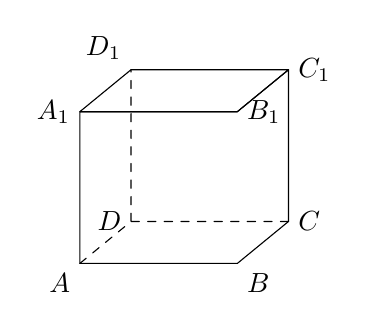
\begin{tikzpicture}[x=1cm,y=0.82cm,line cap=round,line join=round]
\coordinate (A) at (0,0); \coordinate (B) at (2,0); \coordinate (C) at (2.65,0.65); \coordinate (D) at (0.65,0.65);
\coordinate (A1) at (0,2.35); \coordinate (B1) at (2,2.35); \coordinate (C1) at (2.65,3); \coordinate (D1) at (0.65,3);
\draw (A)--(B)--(C)--(C1)--(B1)--(A1)--cycle;
\draw (A1)--(B1) (B1)--(C1) (D1)--(C1) (A1)--(D1);
\draw[dashed] (A)--(D) (D)--(C) (D)--(D1);
\node[below left] at (A) {$A$}; \node[below right] at (B) {$B$};
\node[right] at (C) {$C$}; \node[left] at (D) {$D$};
\node[left] at (A1) {$A_1$}; \node[right] at (B1) {$B_1$};
\node[right] at (C1) {$C_1$}; \node[above left] at (D1) {$D_1$};
\end{tikzpicture}
